 \documentclass [12pt]{article} 

\usepackage {amsmath}
\usepackage {amsthm}
\usepackage {amssymb}
\usepackage {graphicx} 
\usepackage {float}
\usepackage {multirow}
\usepackage {xcolor}
\usepackage {algorithmic}
\usepackage [ruled,vlined,commentsnumbered,titlenotnumbered]{algorithm2e} \usepackage {array} 
\usepackage {booktabs} 
\usepackage {url} 
\usepackage {parskip} 
\usepackage [margin=1in]{geometry} 
\usepackage [T1]{fontenc} 
\usepackage {cmbright} 
\usepackage [many]{tcolorbox} 
\usepackage [colorlinks = true,
            linkcolor = blue,
            urlcolor  = blue,
            citecolor = blue,
            anchorcolor = blue]{hyperref} 
\usepackage {enumitem} 
\usepackage {xparse} 
\usepackage {verbatim}

\DeclareTColorBox {Solution}{}{breakable, title={Solution}} \DeclareTColorBox {Solution*}{}{breakable, title={Solution (provided)}} \DeclareTColorBox {Instruction}{}{boxrule=0pt, boxsep=0pt, left=0.5em, right=0.5em, top=0.5em, bottom=0.5em, arc=0pt, toprule=1pt, bottomrule=1pt} \DeclareDocumentCommand {\Expecting }{+m}{\textbf {[We are expecting:} #1\textbf {]}} \DeclareDocumentCommand {\Points }{m}{\textbf {(#1 pt.)}} 

\begin {document} 

{\LARGE \textbf {COMP 285 (NC A\&T, Spr `22)}\hfill \textbf {Homework 1} } 
\vspace {1em} 
\begin {Instruction} 

\paragraph {Due.} Sunday, January 23th, 2022 @ 11:59 PM!
\end {Instruction} 

\vspace {1em} 
\begin {Instruction} \paragraph {Homework Expectations:} Please see the \href{https://www.comp285.ml/homework/#general-homework-information}{Homework} part of the Course Website (\href{https://www.comp285.ml/policies/#collaboration-policy-and-honor-code}{comp285.ml/policies}) for guidance on what we are looking for in homework solutions. We will grade according to these standards, and you should cite all sources you used outside course material.

\paragraph {What we expect:} Make sure to look at the ``\textbf {We are expecting}'' blocks below each problem to see what we will be grading for in each problem! \end {Instruction}

\vspace {1em} 
\begin {Instruction} 

\paragraph {Exercises.} The following questions are exercises. We suggest you do these on your own. As with any homework question, though, you may ask the course staff for help.

\paragraph {Points} This assignment is worth a total of 100 points.
\end {Instruction} 

\begin{centering}
\section*{Title}
\end{centering}

This course will be a mixture of written homework and coding assignments. Both types of assignments will be submitted through \href{https://www.gradescope.com/courses/350304}{Gradescope}.

In order to reduce the overhead to the course staff, all coding assignments will be released through \href{https://repl.it/}{repl.it}, an in-browser IDE. \textit{This will be the only supported IDE} for the class.

By \textit{supported}, we mean that if you run into issues on \href{https://repl.it/}{repl.it}, the course staff will do everything in their power to resolve them. We \textit{strongly encourage} you to use repl.it for the coding portions of the homework assignments.


\section {Exercise: Setting up repl.it}
\Points{20} As such, the this graded exercise will walk you through setting up your \href{https://repl.it/}{repl.it} account, joining the course, and getting getting your copy of the starter code. Even if you \textbf{do not plan} to use \href{https://repl.it/}{repl.it} for writing/developing your solutions (because you have another preferred IDE), you will use it to obtain your starter code. 

First, let's start by getting you an account and joining the right project:

\begin{enumerate}
    \item If you don't already have a repl.it account with your ``aggies.ncat.edu'' email, head over to the repl.it \href{https://repl.it/}{homepage}. On the top-right, click the `Sign Up' and use your NCAT email address to sign-up.
    \item Complete the registration process (eg, there's a verification email you should get)
    \item Join the @COMP285 Team by following \href{https://repl.it/teams/join/axywewyfiltmqtcgovikrywbqisfdgss-COMP285}{this link}.
\end{enumerate}

Next, let's get your starter code. From your repl.it homepage, you should have a menu down the left-hand side of the page (if not, maybe click the hamburger menu to open it?). Click on "Teams" as shown in Figure \ref{fig:replit_homepage}. You should see `North Carolina A\&T' under `Education', as well as the `COMP 285' Team Project.

Click on `COMP 285', which will take you to the Team Homepage. From there, under `Projects', you should see a link to get started on HW1. Clicking it will give you the starter code, as well as set you up with an online. 

If the above does not work, you can also try going directly to the \href{https://replit.com/team/COMP285/HW1}{project link}.

\begin{figure}[h!]
\centering
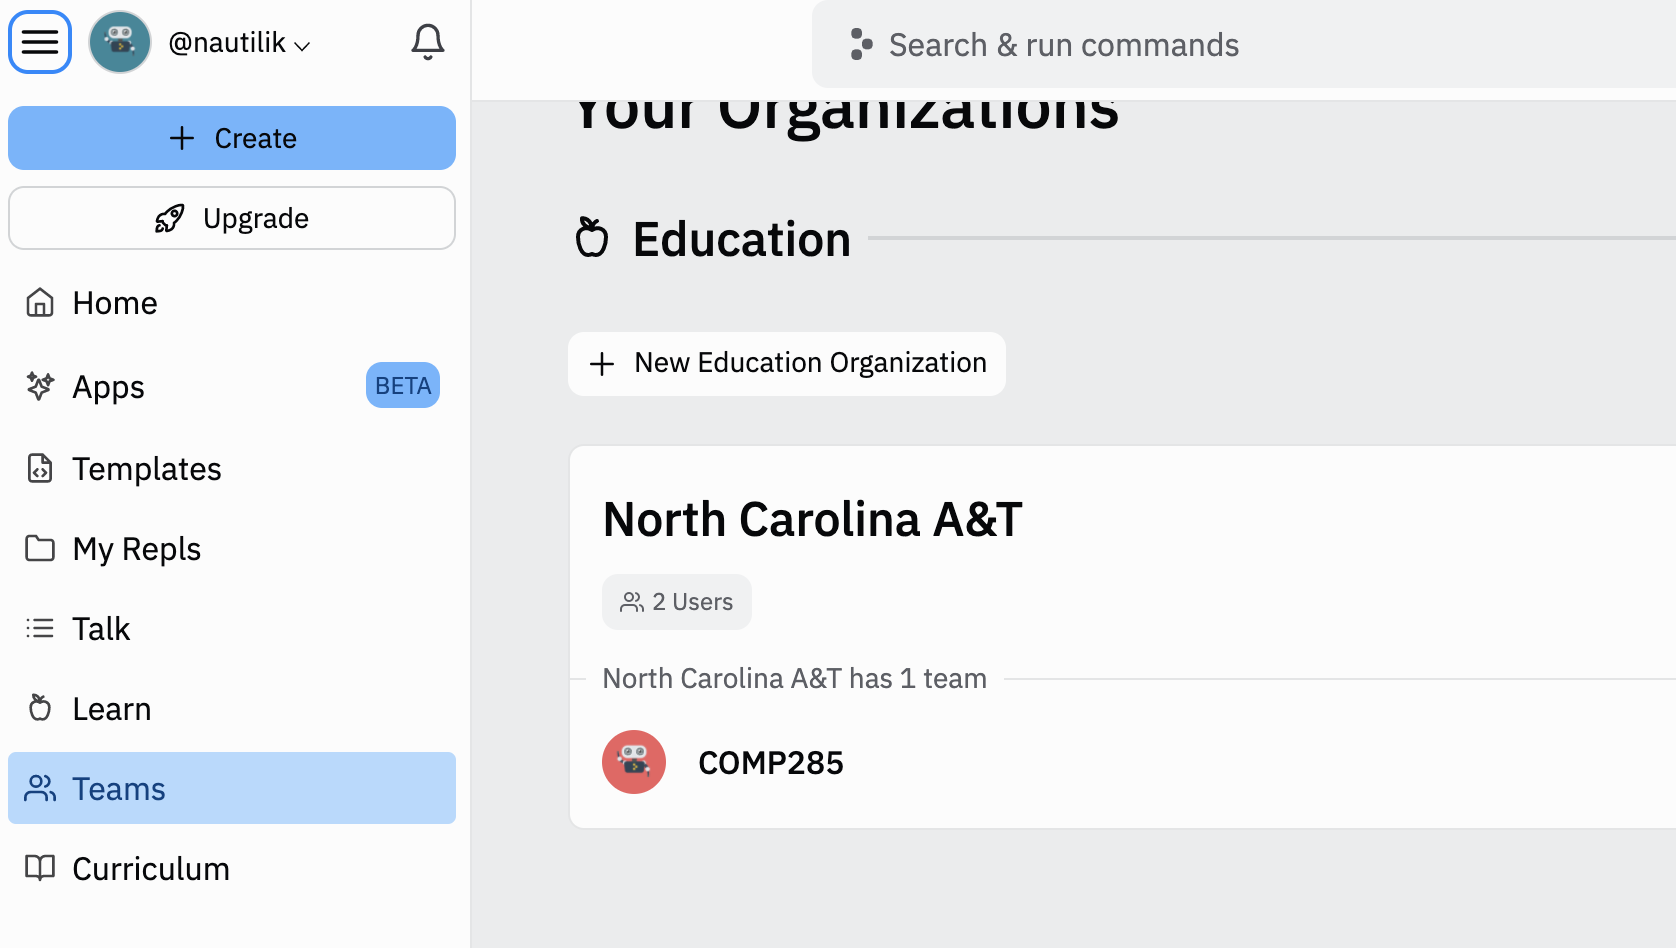
\includegraphics[scale=0.5]{replit}
\caption{Replit Homepage for a student.}
\label{fig:replit_homepage}
\end{figure}

Either way, you should now have the starter code. Clicking the big green button at the top of the IDE will execute the \texttt{main} function defined in `main.cpp'.


\Expecting{You should have a copy of your starter code now available! You can use replit to make edits and run your code. The course staff can see who has started the project, so that is how you'll get credit for this question.}


\section{Exercise}


\end {document} 
